\documentclass{article}
\usepackage{graphicx} % Required for inserting images

\title{Quantum Computing for Drug Discovery Challenge at ICCAD}
\author{Priyabrata Senapati, Waylon Luo and Zixu Wang}
\date{November 2023}

\begin{document}

\maketitle

\section{Introduction}

The rapid advancement of drug discovery relies heavily on state-of-the-art technologies, particularly those that delve into the intricate molecular interactions crucial to medical therapies. Computational methods, prominently featuring machine learning techniques, have gained considerable attention as they unravel complex patterns and optimize solutions. Quantum computing, when coupled with machine learning, holds the potential to revolutionize drug discovery. It not only provides an avenue to overcome challenges considered insurmountable for classical computers but also enhances our ability to predict and comprehend molecular behaviors with unparalleled accuracy\cite{Cao2018}.

In the realm of pharmacology, a pivotal molecule is the hydroxyl cation (·OH). This cation transcends being a mere molecular entity; it serves as a central axis for numerous drug interactions. Its heightened reactivity is associated with oxidative stress, contributing to a spectrum of health conditions ranging from neurodegenerative disorders and cardiovascular diseases to cancers. Beyond its pathogenic implications, the hydroxyl cation plays a crucial role in the effectiveness of many drugs. The advent of quantum computing opens avenues to deepen our comprehension of the interactions and impacts of molecules like the hydroxyl cation, potentially expediting breakthroughs in therapeutic developments.

Given its significance, a detailed understanding of the quantum mechanics of the hydroxyl cation can profoundly influence drug discovery processes. A fundamental starting point involves accurately determining its ground state energy, serving as a foundational element for constructing more intricate drug-cation interactions. However, navigating the quantum realm presents formidable challenges. Current constraints in qubit numbers and quantum error rates hinder comprehensive simulations of larger drug molecules, remaining a distant objective. Here, the manageable size of the hydroxyl cation becomes advantageous. Its relatively compact structure aligns with the current capabilities of quantum computing, making it an ideal candidate for a quantum simulation challenge and, more importantly, charting the course for future research where scalability is a fundamental imperative.

\begin{figure}[h]
\centering
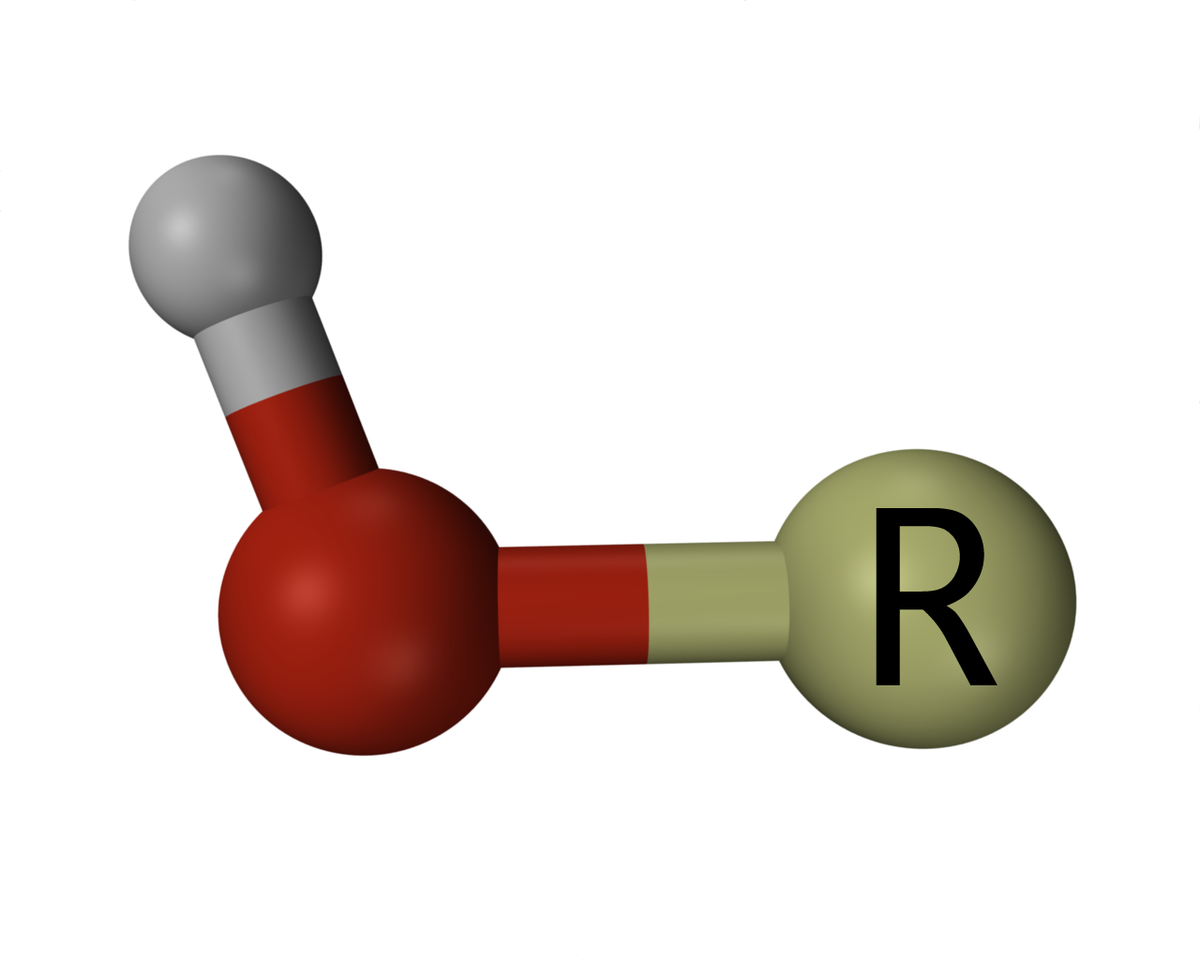
\includegraphics[width=4cm]{Images/Hydroxyl3D.png}
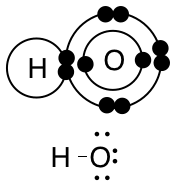
\includegraphics[width=2.5cm]{Images/Hydroxyl-OH.png}
\caption{Molecular Structure of Hydroxyl Cation}
\end{figure}

\section{Objective}

The objective of the 2023 Challenge is to compute the ground state energy of the hydroxyl cation (·OH). The ground state energy of a physical system, particularly in the context of quantum mechanics, is the lowest possible energy that the system can have. In other words, it is the energy of the system when it is in its most stable, lowest-energy configuration.

Our aim is to devise and deploy a functional, open-source protocol capable of autonomously determining the ground state energy of the hydroxyl cation (·OH) using the provided Hamiltonian. Participants are encouraged to explore the design space freely. We suggest an effective qubit mapping strategy achieved through the optimization of co-designed hardware and software. Strategies such as Pauli string grouping and other joint measurement techniques may be implemented to decrease shots on observables, reducing the quantum resource costs. Additionally, employing AI/ML or scientific-based circuit architecture search frameworks can provide a strong basis for enhanced performance. Similarly, AI/ML or scientific-based error mitigation techniques can contribute to achieving superior results.

\section{Data}

%The data used in our work is the hydroxyl oxide molecule. Since the molecule's energy has to be simulated on a quantum computer, the orbital basis of the molecule's electrons are mapped to computational basis by using the Hamiltonian of the molecule.

The data presented in this challenge is centered on drug discovery, specifically delving into the core principles of quantum mechanics governing the hydroxyl cation (·OH). Given its pivotal role in various drug interactions and physiological processes, a nuanced comprehension of the hydroxyl cation is imperative. We used a specialized dataset that is tailored to hydroxyl cation's Hamiltonian. The Hamiltonian is provided as a reference.

The data is presented in text format, with the text file encompassing both the Pauli strings and their corresponding coefficients for the hydroxyl cation's Hamiltonian, employing the Jordan-Wigner mapping \cite{Tranter2018}. While participants are free to employ their preferred tools to generate varied descriptions of the hydroxyl cation's Hamiltonian, it's important to note that we've constrained the fermionic mapping method to adhere to the Jordan-Wigner mapping \cite{Tranter2018}. This constraint specifically entails the utilization of 12 qubits and the inclusion of 631 Pauli strings.

\section{Background}
\subsection{Hamiltonian}
A Hamiltonian is a fundamental concept associated with the energy of a quantum system. The Hamiltonian operator, often denoted as H, is a mathematical representation of the total energy of a quantum system, and it plays a crucial role in quantum mechanics and quantum computing. 

The Hamiltonian describes the dynamics and behavior of a quantum system. It encapsulates the information about the energy levels and the interactions between particles in the system. The time evolution of a quantum state is governed by the Schrödinger equation, which involves the Hamiltonian operator. The Schrödinger equation describes how the quantum state of a system changes over time as a function of the Hamiltonian.

Solving the Schrödinger equation allows one to find the eigenstates (or stationary states) and eigenvalues of the Hamiltonian. The eigenstates represent the possible states of the system, and the corresponding eigenvalues represent the energy levels associated with those states. In variational quantum algorithms like the Variational Quantum Eigensolver (VQE), the Hamiltonian is used to represent the problem at hand, such as simulating the electronic structure of molecules.The Hamiltonian is expressed in terms of Pauli matrices and used to formulate the quantum circuit that represents the evolution of the quantum state. This formulation is known as the qubit Hamiltonian.

\section{Methods}



\section{Results}

\section{Conclusion}
The intersection of quantum computing and drug discovery, as exemplified by the exploration of the hydroxyl cation (·OH) in this challenge, holds tremendous promise for advancing our understanding of molecular interactions and revolutionizing therapeutic development. The rapid progress in drug discovery heavily relies on cutting-edge technologies, and the integration of quantum computing with machine learning presents a transformative approach.

The detailed examination of the hydroxyl cation's quantum mechanics has showcased its significance in pharmacology, not only as a pivotal molecule in drug interactions but also in influencing the effectiveness of various medications. Quantum computing provides a unique opportunity to overcome classical computational limitations, offering avenues to predict and comprehend molecular behaviors with unprecedented accuracy.

The 2023 Challenge, focused on computing the ground state energy of the hydroxyl cation, encourages participants to explore innovative solutions. The emphasis on effective qubit mapping, co-designed hardware and software optimization, and the integration of AI/ML and scientific-based approaches highlights the multifaceted strategies needed for success in quantum simulations.

The provided dataset, centered on the hydroxyl cation's Hamiltonian, underscores the importance of nuanced comprehension in drug discovery. The utilization of specialized data, adhering to the Jordan-Wigner mapping, presents a challenge that aligns with the current capabilities of quantum computing while pushing the boundaries of research.

As the field progresses, addressing challenges such as qubit limitations and quantum error rates remains imperative for comprehensive simulations of larger drug molecules. The manageable size of the hydroxyl cation becomes advantageous in this context, serving as an ideal candidate for quantum simulation challenges and laying the groundwork for scalable solutions in future research.

In summary, the 2023 Challenge provides a platform to advance the synergy between quantum computing and drug discovery. By fostering innovation and collaboration, this endeavor contributes to the ongoing dialogue in quantum chemistry, offering insights that may reshape the landscape of pharmaceutical research and development.

\bibliographystyle{plainurl}
\bibliography{bibliography}

\end{document}
